\documentclass[border=1pt]{standalone}
\usepackage[T1]{fontenc}
\usepackage{mathptmx}
\usepackage{amsmath}
\usepackage{xcolor}
\usepackage{pgfplots}
\usepackage{pgfplotstable}
\pgfplotsset{compat=1.17}
\usepgfplotslibrary{groupplots}
\usetikzlibrary{positioning,calc}
\definecolor{cStd}{RGB}{0,114,178}
\definecolor{cRFM}{RGB}{230,159,0}
\definecolor{cCon}{RGB}{0,158,115}
\definecolor{cML}{RGB}{213,94,0}
\definecolor{cCL}{RGB}{86,180,233}
\definecolor{aHigh}{RGB}{213,94,0}
\definecolor{aReg}{RGB}{0,114,178}
\definecolor{aOcc}{RGB}{0,158,115}
\definecolor{aLap}{RGB}{160,160,160}
\begin{document}
\setlength{\columnwidth}{252pt}\setlength{\textwidth}{516pt}
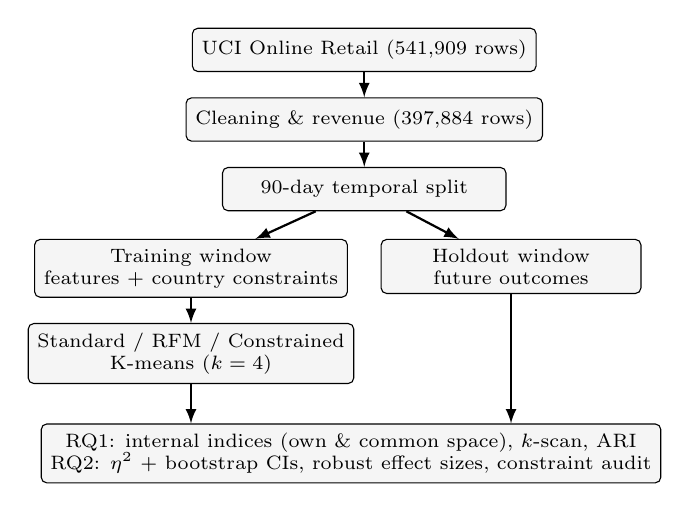
\begin{tikzpicture}[
  node distance=0.32cm,
  box/.style={draw, rounded corners=2pt, align=center, font=\scriptsize,
              minimum width=3.6cm, minimum height=0.55cm, fill=gray!8},
  arr/.style={-latex, thick}]
\node[box] (raw) {UCI Online Retail (541,909 rows)};
\node[box, below=of raw] (clean) {Cleaning \& revenue (397,884 rows)};
\node[box, below=of clean] (split) {90-day temporal split};
\node[box, below left=0.35cm and -1.6cm of split, minimum width=3.3cm] (train)
  {Training window\\features + country constraints};
\node[box, below right=0.35cm and -1.6cm of split, minimum width=3.3cm] (fut)
  {Holdout window\\future outcomes};
\node[box, below=of train, minimum width=3.3cm] (models)
  {Standard / RFM / Constrained\\K-means ($k=4$)};
\node[box, below=0.5cm of $(models.south)!0.5!(fut.south |- models.south)$,
      minimum width=7.2cm] (eval)
  {RQ1: internal indices (own \& common space), $k$-scan, ARI\\
   RQ2: $\eta^2$ + bootstrap CIs, robust effect sizes, constraint audit};
\draw[arr] (raw) -- (clean);
\draw[arr] (clean) -- (split);
\draw[arr] (split) -- (train);
\draw[arr] (split) -- (fut);
\draw[arr] (train) -- (models);
\draw[arr] (models) -- (models |- eval.north);
\draw[arr] (fut) -- (fut |- eval.north);
\end{tikzpicture}
\end{document}
